\section{\primemethodname: Architecting Accelerators via Conservative Models}
\label{sec:method}
%
As shown in Figure~\ref{fig:method}, our method first learns a conservative surrogate model of the optimization objective using the offline dataset. Then, it optimizes this learned model using a discrete optimizer. The optimization process does not require access to a simulator, nor to real-world experiments beyond the initial dataset, except when evaluating the final top-performing $n=256$ designs (Section~\ref{sec:accel}). This is built on the principle of conservative value estimation for offline RL from Chapter ??: while conservative value estimation methods attempt to estimate a pessimistic value-function, we can consider our approach as a special case involving a single decision-making step.

\begin{figure}
    \centering
    \vspace{-0.3cm}
    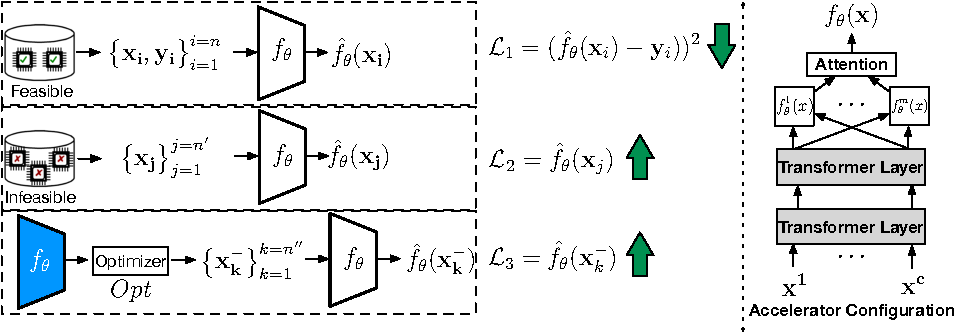
\includegraphics[width=0.7\linewidth]{chapters/prime/figs/overview/mbo-method.pdf}
    \vspace{-0.1cm}
    \caption{\small{Overview of \primemethodname\ which trains a conservative model ${f}_\theta(\rvx_i)$ using Equation~\ref{eqn:final_training}. Our neural net model for ${f}_\theta(\rvx)$ utilizes two transformer layers~\citep{vaswani2017attention}, and a multi-headed architecture which is pooled via a soft-attention layer.}}
    \vspace{-0.3cm}
    \label{fig:method}
\end{figure}

\subsection{Learning Conservative Models Using Logged Offline Data}
Our goal is to utilize a logged dataset of feasible accelerator designs labeled with the desired performance metric (e.g., latency),  $\mathcal{D}_\text{feasible}$, and additional infeasible designs, $\mathcal{D}_\text{infeasible}$ to learn a mapping ${f}_\theta: \mathcal{X} \rightarrow \mathbb{R}$, that maps the accelerator configuration $\rvx$ to its corresponding metric $y$. This learned conservative model can then be optimized by the optimizer. While a straightforward approach for learning such a mapping is to train it via supervised regression (which is equivalent to standard temporal-difference learning for value estimation when considering one-step decision-making scenarios), by minimizing the mean-squared error $\E_{\rvx_i, y_i \sim \mathcal{D}}[(f_\theta(\rvx_i) - y_i)^2]$, as we have seen in this dissertation and in other prior works~\citep{kumar2019model}, such predictive models can arbitrarily overestimate the value of an unseen input $\rvx_i$. This can cause the optimizer to find a solution $\rvx^*$ that performs poorly in the simulator but looks promising under the learned model. We empirically validate this overestimation hypothesis and find it to confound the optimizer in on our problem domain as well (See Figure~\ref{fig:cali_plot} in Appendix). 

To prevent overestimated values at unseen inputs from confounding the optimizer, we follow the conservative value estimation recipe from Chapter ?? (specifically, Equation ??) and train $f_\theta(\rvx)$ with an additional term that explicitly maximizes the function value $f_\theta(\rvx)$ at out-of-distribution $\rvx$ values. Note that instead of minimizing the value $f_\theta(\rvx)$ on unseen $\rvx$, we maximize this value because the problem in Equation ?? requires us to find the minimum of the ground-truth function. Such unseen designs $\rvx$ are ``negative mined'' by running a few iterations of a stochastic optimization procedure that aims to maximize $f_\theta$ in the inner loop. In the context of this single-step decision-making problem, this procedure is analogous to adversarial training~\citep{goodfellow2014explaining}. Equation~\ref{eqn:training} formalizes this objective:
\newcommand{\editcolor}{black}
\begin{equation}
\label{eqn:training}
    \theta^* := \arg \min_\theta~~ \mathcal{L}(\theta):= \E_{\rvx_i, y_i \sim \mathcal{D}_{\text{feasible}}} \left[ (f_\theta(\rvx_i) - y_i)^2 \right] - \alpha \E_{\rvx^{-}_i \sim \textcolor{\editcolor}{\mathrm{Opt}(f_\theta)}} \left[f_\theta(\rvx^-_i) \right].
\end{equation}
$\rvx^{-}_i$ denotes the negative samples produced from an optimizer $\mathrm{Opt}(\cdot)$ that attempts to maximize the current learned objective model, $f_\theta$. We will discuss our choice of $\mathrm{Opt}$ in the Appendix Section~\ref{app:details}.  
 
\subsection{Incorporating Design Constraints by Training on Infeasible Points}
While conservative value estimation methods simply discuss how we can optimize Equation~\ref{eqn:training} by learning a conservative model, this is not enough when optimizing over accelerators, as we will also show empirically (Appendix~\ref{app:additional_experiments}).
This is because explicitly minimizing for out-of-distribution designs does not provide any information about accelerator design constraints. Fortunately, this information can be provided by infeasible points, $\mathcal{D}_\text{infeasible}$. The training procedure in Equation~\ref{eqn:training} provides a simple way to do incorporate such infeasible points: we simply incorporate $\rvx'_i \sim \mathcal{D}_{\text{infeasible}}$ as additional out-of-distribution samples and maximize the prediction at these points.
This gives rise to our final objective:
\begin{equation}
\label{eqn:final_training}
    \min_\theta~~ \mathcal{L}^\text{inf}(\theta) := \mathcal{L}(\theta)
    - \textcolor{blue}{\beta \E_{\rvx'_i \sim \mathcal{D}_{\text{infeasible}}}\left[ f_\theta(\rvx'_i) \right]}
\end{equation}

\subsection{Optimizing Multiple Applications and Zero-Shot Design}
%
One of the central benefits of an offline learning approach is that it enables learning powerful models that generalize over the space of applications, potentially being effective for new unseen application domains. In our experiments, we evaluate \primemethodname\ on designing accelerators for multiple applications denoted as $k=1, \cdots, K$, jointly or for a novel unseen application. In this case, we utilized a dataset $\mathcal{D} = \{\mathcal{D}_1, \cdots, \mathcal{D}_K\}$, where each $\mathcal{D}_k$ consists of a set of accelerator designs, annotated with the latency value and the feasibility criterion for a given application $k$. While there are a few overlapping designs in different parts of the dataset annotated for different applications, most of the designs only appear in one part. To train a single conservative model $f_\theta(\cdot)$ for multiple applications, we extend the training procedure in Equation~\ref{eqn:final_training} to incorporate \textit{context vectors} $\rvc_k \in \mathbb{R}^d$ for various applications driven by a list of application properties in Table~\ref{tab:models}. A context vector is akin to a state in the context of full sequential reinforcement learning. 

The learned function in this setting is now conditioned on the context $f_\theta(\rvx, \rvc_k)$. We train $f_\theta$ via the objective in Equation~\ref{eqn:final_training}, but in expectation over all the contexts and their corresponding datasets: $\min_\theta \E_{\textcolor{blue}{k \sim [K]}}\left[\mathcal{L}^\text{inf}_k(\theta)\right]$. Once such a contextual model is learned, we can either optimize the average models across a set of contexts $\{\rvc_i, \rvc_2, \cdots, \rvc_n\}$ to obtain an accelerator that is optimal for multiple applications simultaneously on an average (``multi-model'' optimization), or optimize this contextual model for a novel context vector, corresponding to an unseen application (``zero-shot'' generalization). In this case, \primemethodname\ is not allowed to train on any data corresponding to this new unseen application.  While such zero-shot generalization might appear surprising at first, note that the context vectors are not simply one-hot vectors, but consist of parameters with semantic information, which the conservative model can generalize over.

~

\niparagraph{Learned conservative model optimization.} Prior work~\citep{yazdanbakhsh2021apollo} has shown that the most effective optimizers for accelerator design are meta-heuristic/evolutionary optimizers. We therefore choose to utilize, firefly~\citep{yang2010nature,yang2010eagle,liu2013adaptive} to optimize our conservative model. This algorithm maintains a set of optimization candidates (a.k.a. ``fireflies'') and jointly update them towards regions of low objective value, while adjusting their relative distances appropriately to ensure multiple high-performing, but diverse solutions. We discuss additional details in Appendix~\ref{sec:practical_implementation}.

~

\niparagraph{Cross validation: which model and checkpoint should we evaluate?} Similarly to supervised learning, models trained via Equation~\ref{eqn:final_training} can overfit, leading to poor solutions. Thus, we require a procedure to select which hyperparameters and checkpoints should actually be used for the design. This is crucial, because we cannot arbitrarily evaluate as many models as we want against the simulator. While effective methods for model selection have been hard to develop in offline reinforcement learning~\citep{trabucco2021conservative,trabucco2021designbench}, we devised a simple scheme using a validation set for choosing the values of $\alpha$ and $\beta$ (Equation~\ref{eqn:final_training}), as well as which checkpoint to utilize for generating the design. For each training run, we hold out the best 20\% of the points out of the training set and use them \textit{only} for cross-validation as follows. Typical cross-validation strategies in supervised learning involve tracking validation error (or risk), but since our model is trained conservatively, its predictions may not match the ground truth, making such validation risk values unsuitable for our use case. Instead, we track Kendall's ranking correlation between the predictions of the learned model $f_\theta(\rvx_i)$ and the ground truth values $y_i$ (Appendix~\ref{app:details}) for the held-out points for each run.
We pick values of $\alpha$, $\beta$ and the checkpoint that attain the highest validation ranking correlation.
We present the pseudo-code for \primemethodname\ (Algorithm~\ref{alg:prime}) and implementation details in Appendix~\ref{sec:practical_implementation}.